% =====================================================================
% ICAIF 2026 / ACM sigconf anonymous submission build
% Primary target: ACM International Conference on AI in Finance (ICAIF) 2026
% =====================================================================
% For double-blind submission upload, re-add the "anonymous" option:
%   \documentclass[sigconf,anonymous,nonacm]{acmart}
\documentclass[sigconf,nonacm]{acmart}

\settopmatter{printacmref=false}
\renewcommand\footnotetextcopyrightpermission[1]{}
\pagestyle{plain}

% acmart already loads natbib, url, hyperref, amsmath, and graphicx.
\usepackage{booktabs}
\usepackage{multirow}
\usepackage{algorithm}
\usepackage{algorithmic}
\usepackage{xcolor}
\usepackage{microtype}
\usepackage{tikz}
\usetikzlibrary{positioning, arrows.meta, shapes.geometric, calc}

\newtheorem{proposition}{Proposition}
\graphicspath{{figures/}{../results/figures/}}

\acmConference[ICAIF '26]{The 7th ACM International Conference on AI in Finance}{November 14--17, 2026}{Milan, Italy}
\acmBooktitle{ICAIF '26: The 7th ACM International Conference on AI in Finance, November 14--17, 2026, Milan, Italy}
\acmYear{2026}
\copyrightyear{2026}
\acmDOI{}
\acmISBN{}

\title{DHRP: A Differentiable Hierarchical Risk Parity Architecture and Multi-Universe Portfolio Benchmark}

\author{Jose Luis Amador Jaime}
\affiliation{\institution{Independent Researcher}\country{USA}}

\begin{document}
\begin{abstract}
We introduce \textbf{DHRP}, a differentiable extension of Hierarchical Risk
Parity \citep{LopezdePrado2016} that replaces hard agglomerative clustering
and recursive bisection with a temperature-scaled soft-gating tree, and
\textbf{DHRP-8}, the first multi-universe portfolio benchmark reporting
Probabilistic Sharpe Ratios \citep{Bailey2012PSR} and Fama--French factor
alphas under 10-seed protocols across eight ETF asset classes.
DHRP achieves out-of-sample Sharpe ratios of $\mathbf{1.304 \pm 0.10}$ on
commodities ($\text{PSR}=0.999$) and $\mathbf{1.290 \pm 0.05}$ on crypto
($\text{PSR}=0.991$), beating classical HRP in six of eight universes.
Fama--French 3-factor alpha on commodities is $6.3\%$ ($t=1.58$, not
significant), so the strongest claim is robust positive sample Sharpe rather
than significant factor alpha. DHRP underperforms mean-variance in
equity-heavy universes where factor exposures dominate.
Cross-modal LLM augmentation via FinBERT \citep{Huang2023} embeddings
provides \emph{no statistical benefit} under multi-seed reporting,
regressing $-0.57$ Sharpe in commodities and $-0.21$ in developed markets.
This honest negative ablation joins a growing benchmark literature
\citep{Tan2024AreLMs,Chen2025StockBench} cautioning against single-seed
LLM-finance claims. We release the 8-universe dataset (Croissant~1.1
metadata), multi-seed checkpoints, and a single-command reproduction pipeline.
\end{abstract}
\maketitle


\section{Introduction}
\label{sec:intro}

Portfolio optimization sits at the intersection of statistical estimation
and constrained decision-making. Mean--variance optimization
\citep{Markowitz1952} is fragile to estimation error
\citep{DeMiguel2009,Ledoit2004}; Hierarchical Risk Parity (HRP)
\citep{LopezdePrado2016} sidesteps this by routing capital down a binary
tree built from agglomerative clustering of correlation distances. HRP
has become a practitioner standard, but its hard clustering and
recursive bisection are non-differentiable, blocking joint training
with upstream feature extractors. Differentiable optimization layers
\citep{Amos2017,Agrawal2019,Bolte2021,Pan2024BPQP}, soft decision trees
\citep{FrosstHinton2017,Popov2020NODE,Mao2025DiffTree}, and gated
mixture-of-experts \citep{Shazeer2017} have shown that hierarchical
routing can be made differentiable while retaining the inductive bias
that makes trees interpretable.

We bring these architectures to portfolio allocation. \textbf{DHRP}
replaces HRP's clustering and bisection with a temperature-scaled
soft-gating tree, enabling end-to-end gradient training while retaining
an HRP-like inductive bias. It is an HRP-inspired differentiable
relaxation; we do not claim the hard-routing limit reproduces the full
classical HRP algorithm. We evaluate eight headline methods across
\textbf{eight asset universes} with multi-seed reporting (10 seeds,
mean$\pm$std, Probabilistic Sharpe Ratios) and Fama--French factor
alphas. We also test cross-modal LLM augmentation (LLM-DHRP)
fusing FinBERT \citep{Huang2023} embeddings of asset-attributed news,
and find that text augmentation provides \emph{no statistical lift}
under multi-seed reporting---joining a growing benchmark literature
\citep{Tan2024AreLMs,Chen2025StockBench,Xie2024FinBen} that cautions
against single-seed claims of LLM benefit in finance.

\paragraph{Contributions.}
\begin{enumerate}\itemsep0.05em
\item \textbf{DHRP architecture:} a
  temperature-scaled soft-gating tree that provides a differentiable
  HRP-like allocation bias without asserting exact classical-HRP
  equivalence.
\item \textbf{DHRP-8 benchmark:} an
  8-universe portfolio evaluation framework (DM, EM, commodities,
  sectors, global multi-asset, factors, crypto, bonds) with eight
  headline methods, 12 implemented allocators, 10-seed reporting, PSR,
  Fama--French factor alphas, transaction-cost sensitivity, and
  Croissant~1.1 metadata.
\item \textbf{Empirical findings:} DHRP achieves PSR $> 0.99$ on commodities
  ($1.30 \pm 0.10$ Sharpe) and crypto ($1.29 \pm 0.05$), beats
  classical HRP in six of eight universes, and ties or beats all classical
  baselines in DM. Mean-variance dominates equity-heavy global
  multi-asset. LLM augmentation regresses ($-0.21$ Sharpe in DM,
  $-0.57$ in commodities) under multi-seed reporting.
\end{enumerate}


\section{Related Work}
\label{sec:related}

\paragraph{HRP and differentiable optimization.}
HRP \citep{LopezdePrado2016} replaces inverse-covariance MV with
single-linkage agglomerative clustering and recursive bisection, with
extensions to alternative linkages \citep{Raffinot2018} and risk-parity
budgeting \citep{Roncalli2013}. Differentiable optimization layers
\citep{Amos2017,Agrawal2019,Bolte2021} embed structured decision-making
in neural networks; BPQP \citep{Pan2024BPQP} applies this to mean--variance
portfolios with end-to-end Sharpe training, and \citet{Lin2024MSparse}
solve $m$-sparse Sharpe with theoretical guarantees. DHRP imposes
HRP's hierarchical inductive bias instead of solving a generic convex
program, which empirically wins in low-correlation regimes
(Results section).

\paragraph{Soft trees and decision-focused learning.}
Soft decision trees \citep{FrosstHinton2017,Popov2020NODE,Hazimeh2020TreeEnsemble}
and gated mixture-of-experts \citep{Shazeer2017} demonstrate that
hierarchical routing can be made differentiable. \citet{Mao2025DiffTree}
provide a recent NeurIPS spotlight on differentiable trees via
ReLU+Argmin reformulation. Decision-focused learning
\citep{Wilder2019,Elmachtoub2022SPO,Donti2017} optimizes prediction for
the downstream optimization task; recent finance applications include
deep declarative risk budgeting \citep{ParraDiaz2025} and decision-
focused minimum-variance \citep{KimLee2025DFL}. DHRP is decision-
focused by construction.

\paragraph{LLMs in finance and benchmark precedents.}
FinBERT \citep{Huang2023}, BloombergGPT \citep{Wu2023BloombergGPT}, and
sentiment-augmented RL \citep{Kirtac2025} explore LLM-portfolio fusion.
However, recent benchmark papers consistently document that LLM
competence on text tasks does not transfer to financial decisions:
StockBench \citep{Chen2025StockBench} shows most LLM agents fail to
beat buy-and-hold; FinBen \citep{Xie2024FinBen} finds LLM weakness in
forecasting; \citet{Tan2024AreLMs} (NeurIPS 2024 Spotlight) show that
removing the LLM component improves time-series forecasting. Our
LLM-DHRP ablation extends this evidence
to hierarchical portfolio allocation.

\paragraph{Multi-seed and PSR reporting.}
Probabilistic Sharpe Ratio \citep{Bailey2012PSR} and Deflated Sharpe
\citep{Bailey2014DSR} correct Sharpe significance for sample size,
non-Normality, and selection bias. Recent ML-finance work reports
mean$\pm$std over 10--100 seeds \citep{ParraDiaz2025,Pan2024BPQP};
BetterBench \citep{Reuel2024BetterBench} explicitly critiques benchmarks
without multi-seed error bars. DHRP-8 adopts both standards.


\section{Method}
\label{sec:method}

We follow classical HRP's correlation-distance clustering and recursive risk budgeting, and present DHRP and LLM-DHRP here. The full architecture is shown in
Figure~\ref{fig:arch}.
% TikZ architecture diagram for DHRP + LLM-DHRP (inlined into main.tex).
\begin{figure*}[t]
\centering
\resizebox{\textwidth}{!}{%
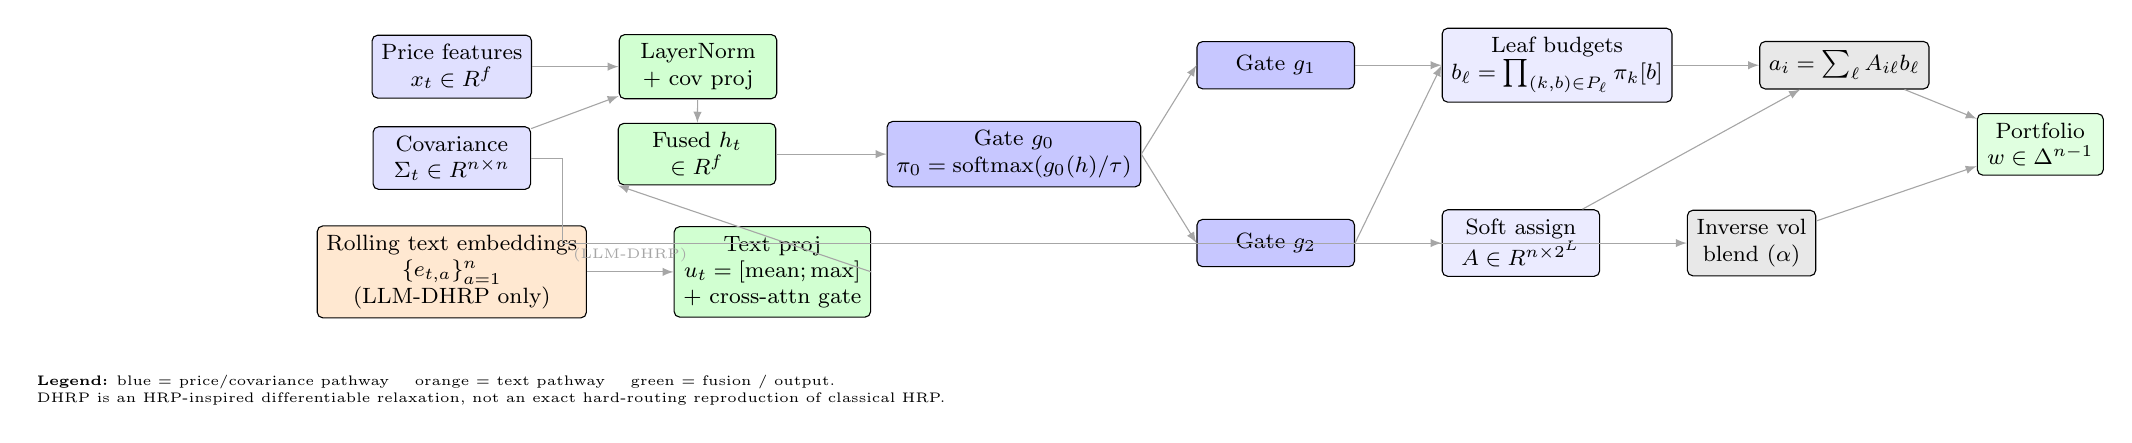
\begin{tikzpicture}[
    node distance=0.9cm,
    every node/.style={font=\small},
    box/.style={draw, rounded corners=2pt, minimum width=2.0cm, minimum height=0.6cm,
                align=center, font=\footnotesize},
    txt/.style={box, fill=orange!18},
    price/.style={box, fill=blue!12},
    cov/.style={box, fill=blue!12},
    fuse/.style={box, fill=green!18},
    tree/.style={box, fill=blue!22},
    outbox/.style={box, fill=gray!18, minimum width=1.6cm},
    arrow/.style={->, >=latex, thin, gray!70},
    dashedarrow/.style={->, >=latex, thin, gray!50, dashed},
]

% --- Inputs (left column) ---
\node[price]                              (x)   {Price features\\ $x_t \in \mathbb{R}^{f}$};
\node[cov,    below=0.35cm of x]          (S)   {Covariance\\ $\Sigma_t \in \mathbb{R}^{n\times n}$};
\node[txt,    below=0.45cm of S]          (T)   {Rolling text embeddings\\ $\{e_{t,a}\}_{a=1}^n$\\ (LLM-DHRP only)};

% --- Feature fusion (middle column) ---
\node[fuse,   right=1.1cm of x]           (norm) {LayerNorm\\ + cov proj};
\node[fuse,   right=1.1cm of T]           (txp)  {Text proj\\ $u_t=[\mathrm{mean};\mathrm{max}]$\\ + cross-attn gate};
\node[fuse,   right=1.1cm of S, yshift=0.05cm] (h) {Fused $h_t$\\ $\in \mathbb{R}^{f}$};

% --- Soft-gating tree (right column) ---
\node[tree,   right=1.4cm of h]           (g0)  {Gate $g_0$\\ $\pi_0 = \mathrm{softmax}(g_0(h)/\tau)$};
\node[tree,   below right=0.4cm and 0.7cm of g0] (g2) {Gate $g_2$};
\node[tree,   above right=0.4cm and 0.7cm of g0] (g1) {Gate $g_1$};

% --- Leaf budgets + assignment + output ---
\node[box,    fill=blue!8, right=1.1cm of g1] (leaves) {Leaf budgets\\ $b_\ell = \prod_{(k,b)\in P_\ell} \pi_k[b]$};
\node[box,    fill=blue!8, right=1.1cm of g2] (assign) {Soft assign\\ $A \in \mathbb{R}^{n\times 2^L}$};
\node[outbox,    right=1.1cm of leaves]      (alloc) {$a_i = \sum_\ell A_{i\ell} b_\ell$};
\node[outbox,    right=1.1cm of assign]      (vol)   {Inverse vol\\ blend ($\alpha$)};
\node[outbox,    fill=green!12, below right=0.3cm and 0.6cm of alloc] (w) {Portfolio\\ $w \in \Delta^{n-1}$};

% --- Arrows ---
\draw[arrow] (x) -- (norm);
\draw[arrow] (S) -- (norm);
\draw[arrow] (T) -- (txp) node[midway, above, font=\tiny]{(LLM-DHRP)};
\draw[arrow] (norm) -- (h);
\draw[arrow] (txp.east) -- (h.south west);
\draw[arrow] (h) -- (g0);
\draw[arrow] (g0.east) -- (g1.west);
\draw[arrow] (g0.east) -- (g2.west);
\draw[arrow] (g1.east) -- (leaves.west);
\draw[arrow] (g2.east) -- (leaves.west);
\draw[arrow] (g2.east) -- (assign.west);
\draw[arrow] (leaves) -- (alloc);
\draw[arrow] (assign) -- (alloc);
\draw[arrow] (S.east) -- ++(0.4,0) |- (vol.west);
\draw[arrow] (alloc) -- (w);
\draw[arrow] (vol)   -- (w);

% --- Legend (compact) ---
\node[below=0.6cm of T, xshift=0.5cm, font=\tiny, align=left] {%
  \textbf{Legend:} blue = price/covariance pathway \quad orange = text pathway \quad green = fusion / output.\\
  DHRP is an HRP-inspired differentiable relaxation, not an exact hard-routing reproduction of classical HRP.};
\end{tikzpicture}%
}
\caption{DHRP and LLM-DHRP architecture. Price features, covariance,
and (optional) global text summaries are fused via LayerNorm and a
gated cross-attention residual into $h_t$, which routes through a
temperature-scaled binary gating tree. Leaf budgets are combined with a
learned soft assignment matrix and blended with inverse-volatility
weights to produce portfolio weights $w \in \Delta^{n-1}$.}
\label{fig:arch}
\end{figure*}


\subsection{DHRP: differentiable soft-gating tree}
\label{sec:dhrp_layer}

DHRP maps a feature vector $x_t \in \mathbb{R}^f$ and an annualized
covariance $\Sigma_t \in \mathbb{R}^{n \times n}$ to portfolio weights
$w_t \in \Delta^{n-1}$ via four learnable components.

\paragraph{Feature fusion.}
A covariance projection MLP $f_{\text{cov}}: \mathbb{R}^{n^2} \to \mathbb{R}^f$
encodes the flattened normalized covariance, then layer-norm fuses with
price features:
\begin{equation}
h_t = \mathrm{LayerNorm}\left(x_t + f_{\text{cov}}\!\left(
\mathrm{vec}(\Sigma_t)/(\|\Sigma_t\|_\infty + \epsilon)\right)\right).
\end{equation}

\paragraph{Soft-gating tree.}
A perfect binary tree of depth $L$ has $2^L$ leaves and $2^L-1$ internal
nodes. Each internal node $k$ has a gate $g_k: \mathbb{R}^f \to \mathbb{R}^2$
with temperature-scaled softmax:
\begin{equation}
\pi_k = \mathrm{softmax}(g_k(h_t) / \tau_k),
\quad \tau_k = \exp(\theta_{\tau,k}) \in (0.1, 5.0].
\label{eq:gates}
\end{equation}
Leaf budget for leaf $\ell$ along path $P_\ell$ is
$p_\ell = \prod_{(k, b) \in P_\ell} \pi_k[b]$, normalized by a learned
prior $\beta = \mathrm{softmax}(\theta_\beta)$:
$b_\ell = \beta_\ell p_\ell / \sum_j \beta_j p_j$.

\paragraph{Soft asset assignment and volatility blending.}
A learnable matrix $A \in \mathbb{R}^{n \times 2^L}$ row-normalizes via
softmax; asset $i$ receives $a_i = \sum_\ell \mathrm{softmax}(A_{i,:})_\ell\, b_\ell$.
Final weights blend with inverse-volatility:
\begin{equation}
w_i = \alpha \cdot a_i + (1-\alpha) \cdot \frac{1/\sigma_i}{\sum_j 1/\sigma_j},
\qquad \alpha = \sigma(\theta_\alpha),
\label{eq:blend}
\end{equation}
followed by non-negativity clipping and re-normalization.

\paragraph{Loss.}
Multi-objective: CRRA utility, smooth Sharpe, HRP regularization
(curriculum-scheduled $\lambda_h: 0.3 \to 0.05$ over training), risk
penalty, concentration (HHI), and turnover penalty:
\begin{align}
\mathcal{L} &= -(\mathrm{CRRA} + \mathrm{Sharpe} + \lambda_e \mathrm{Entropy}) \notag\\
&\quad + \lambda_h \|w - w_{\text{HRP}}\|_2^2 + \lambda_r w^\top \Sigma w \notag\\
&\quad + \lambda_c \mathrm{HHI}(w) + \lambda_t \mathrm{TO}(w).
\end{align}
The HRP regularizer warm-starts from classical HRP weights, providing
the inductive bias that anchors the relaxation.

\paragraph{Architecture scope.}
DHRP is an HRP-inspired differentiable allocator, not a differentiable
implementation of the full L\'opez de Prado algorithm. The implemented
tree sends mass through temperature-scaled gates, learns soft
asset-to-leaf assignments, and blends the resulting budget with
inverse-volatility weights. This architecture can approximate
HRP-like allocations when its split budgets, assignments, and
volatility blend are constrained to match a fixed HRP solution, but its
hard-routing limit does not generally reproduce recursive HRP
bisection across all subtrees. Exact reproduction would require an
architecture in which each internal node emits split budget proportions
for both children.

A row-wise entropy-regularized interpretation of the soft assignment matrix connects the assignment to the Sinkhorn literature, although our implementation enforces only row-stochasticity rather than the full bi-stochastic Sinkhorn iteration.

\subsection{LLM-DHRP: text-augmented allocation}
\label{sec:llm_dhrp_arch}

LLM-DHRP augments the price pathway with a single text summary vector
per timestep, built from per-asset news headlines. For each asset $a$
we collect headlines within a 90-day rolling window, encode each
headline with FinBERT \citep{Huang2023} ($d_T = 768$), and average
headline embeddings within the asset window to obtain
$e_{t,a}\in\mathbb{R}^{d_T}$. We normalize
$\tilde e_{t,a}=e_{t,a}/(\|e_{t,a}\|_2+\epsilon)$ and form the global
summary
\[
u_t =
\left[
\frac{1}{n}\sum_{a=1}^{n}\tilde e_{t,a};
\max_{a=1,\ldots,n}\tilde e_{t,a}
\right]\in\mathbb{R}^{2d_T}.
\]
A TextProjection MLP maps $u_t$ to $\mathbb{R}^f$, and a gated residual
fuses it into the price pathway:
\begin{equation}
\hat h_t = h_t + g_{\text{text}} \cdot
\mathrm{TextProj}(u_t),
\quad g_{\text{text}} = \sigma(\theta_g - 1.0),
\end{equation}
with gate bias $-1.0$ initially suppressing text. Modality dropout
(probability 0.1) randomly masks the text branch during training. We
use a two-phase warm-start: phase~1 freezes price-pathway parameters
and trains text/fusion only; phase~2 unfreezes all with reduced
learning rate; detailed hyperparameters are given in the supplementary material.

We deliberately use a global text summary rather than asset-token
cross-attention. Per-asset headline coverage in our universes is
sparse and skewed toward a few mega-cap names, and pilots with
asset-token attention exhibited high seed-to-seed variance dominated by
coverage gaps rather than text signal. The negative ablation in
the LLM ablation section should therefore be read as a
``does global FinBERT summary help DHRP'' result, not as a verdict on
all possible per-asset text architectures.


\section{The DHRP-8 Benchmark}
\label{sec:benchmark}

DHRP-8 evaluates portfolio allocation across eight asset universes,
eight headline methods, 12 implemented allocators, and a five-family statistical battery. Detailed protocol
specifications and the full per-universe asset list are given in the supplementary material.

\paragraph{Universes (8 total).}
Equity: developed markets (DM, 10 ETFs), emerging markets (EM, 10), US
sectors (10), global multi-asset (10), factor ETFs (10).
Non-equity: commodities (10), crypto (10, post-2020 history), bonds
(10). All ETFs are publicly traded on US exchanges with $\geq$12 years
of daily history (crypto: 2020--2026 only).

\paragraph{Methods.}
Classical: equal-weight (EW), mean--variance (MV), minimum-variance
(MINVAR), risk parity (RP), maximum diversification (MAXDIV),
hierarchical risk parity (HRP). DHRP and LLM-DHRP complete the eight
headline methods. Additional implemented allocators--MLP with
covariance-projection, Portfolio Transformer \citep{KisielGorse2022},
PPO, and DFL mirroring \citet{KimLee2025DFL}--are reported in
supplementary/appendix experiments where evaluated.

\paragraph{Multi-seed protocol.}
Every neural method is trained independently across $S = 10$ seeds
$\{0, \ldots, 9\}$ and backtested over the OOS window 2020-07 to
2026-04 with universe-specific rebalance frequency (5 days for
commodities and crypto; 21 days otherwise). Per-method metrics are
reported as mean$\pm$std across seeds; classical baselines are
deterministic and reported as a single value. Models train on
2012--2020-06 with a 5-day purge gap to prevent train/test leakage.

\paragraph{Statistical battery.}
We report (i)~Probabilistic Sharpe Ratio \citep{Bailey2012PSR}
(probability the true Sharpe exceeds zero, sample-corrected for skew
and kurtosis); (ii)~Newey--West HAC t-statistics
\citep{NeweyWest1987}; (iii)~Fama--French 3 + 5 factor
\citep{FamaFrench2015} and momentum \citep{Carhart1997} regression
alphas; (iv)~stationary
block bootstrap \citep{PolitisRomano1994} pairwise Sharpe-difference
tests with Holm--Bonferroni \citep{Holm1979} and Diebold--Mariano
\citep{DieboldMariano1995} forecast accuracy; (v)~SPA \citep{Hansen2005}
and MCS \citep{HansenLundeNason2011} multi-method tests at
$\alpha = 0.05$.

\paragraph{Reproducibility.}
We release Croissant 1.1 metadata \citep{Akhtar2024Croissant} including
license, schema, train/test splits, and Responsible-AI annotations
covering survivorship bias and data-leakage warnings; the full metadata is included in the supplementary material. The supplementary contains
\texttt{requirements-frozen.txt}, a single-command \texttt{reproduce\_all.sh}
pipeline, and an anonymous code release URL.


\section{Results}
\label{sec:results}

\subsection{Multi-universe Sharpe summary}
\label{sec:results_main}

Table~\ref{tab:headline} reports the headline result. DHRP achieves
PSR $> 0.95$ in commodities ($1.30 \pm 0.10$, PSR $0.999$), crypto
($1.29 \pm 0.05$, PSR $0.991$), and is borderline in sectors (PSR
$0.946$) and factors ($0.949$). DHRP is the best risk-parity-family
method in DM ($0.446 \pm 0.06$ vs.\ HRP $0.216$, EW $0.255$). MV
dominates global multi-asset (Sharpe $0.99$, PSR $0.99$); all methods
bleed in bonds during the 2022--2023 rate-hike period.

% Auto-generated by scripts/generate_paper_tables.py — do not hand-edit
\begin{table*}[t]
\caption{Mean$\pm$std out-of-sample Sharpe across 10 seeds with Probabilistic Sharpe Ratio in brackets. Bold marks best method per universe; $\ast$ marks PSR $> 0.95$. Classical baselines are deterministic (no std).}
\label{tab:headline}
\centering
\setlength{\tabcolsep}{3pt}
\resizebox{\textwidth}{!}{%
\begin{tabular}{lcccccccc}
\toprule
Method & DM & EM & CMD & Sect & Glb & Fact & Cry & Bnd \\
\midrule
EW & 0.255 [0.730] & 0.479 [0.875] & 0.769 [0.967$^{\ast}$] & 0.706 [0.955$^{\ast}$] & 0.559 [0.911] & 0.666 [0.945] & 1.094 [0.978$^{\ast}$] & -1.021 [0.007] \\
MV & 0.333 [0.788] & \textbf{0.660 [0.943]} & 0.408 [0.834] & \textbf{0.861 [0.980$^{\ast}$]} & \textbf{0.994 [0.990$^{\ast}$]} & 0.380 [0.819] & 1.107 [0.979$^{\ast}$] & -0.907 [0.014] \\
MINVAR & -0.711 [0.036] & 0.286 [0.754] & 0.958 [0.989$^{\ast}$] & 0.423 [0.844] & -0.749 [0.036] & 0.493 [0.881] & 0.603 [0.864] & -2.205 [0.000] \\
MAXDIV & -0.456 [0.131] & 0.340 [0.793] & 0.828 [0.976$^{\ast}$] & 0.732 [0.960$^{\ast}$] & 0.081 [0.577] & 0.652 [0.941] & 1.020 [0.969$^{\ast}$] & -1.892 [0.000] \\
RP & 0.001 [0.501] & 0.437 [0.853] & 1.106 [0.991$^{\ast}$] & 0.666 [0.945] & 0.216 [0.699] & 0.670 [0.946] & 1.079 [0.976$^{\ast}$] & -1.525 [0.000] \\
HRP & 0.216 [0.698] & 0.415 [0.841] & 0.971 [0.990$^{\ast}$] & 0.698 [0.953$^{\ast}$] & 0.227 [0.708] & \textbf{0.704 [0.955$^{\ast}$]} & 1.039 [0.972$^{\ast}$] & -1.176 [0.002] \\
DHRP & \textbf{$0.446{\pm}0.056$ [0.856]} & $0.469{\pm}0.004$ [0.870] & \textbf{$1.304{\pm}0.095$ [0.999$^{\ast}$]} & $0.677{\pm}0.050$ [0.946] & $0.357{\pm}0.092$ [0.799] & $0.682{\pm}0.033$ [0.949] & \textbf{$1.290{\pm}0.052$ [0.991$^{\ast}$]} & \textbf{$-0.896{\pm}0.055$ [0.016]} \\
LLM-DHRP & $0.239{\pm}0.119$ [0.712] & $0.474{\pm}0.005$ [0.872] & $0.738{\pm}0.104$ [0.956$^{\ast}$] & --- & --- & --- & --- & --- \\
\bottomrule
\end{tabular}%
}
\end{table*}


\subsection{Factor regression alphas}
\label{sec:results_alphas}

In commodities, DHRP achieves a Fama--French 3-factor annualized alpha
of $6.3\%$ ($t=1.58$, not significant at the 5\% level), with the next-
best classical baseline (MINVAR) at $7.3\%$ ($t=2.25$). LLM-DHRP attains
a higher FF3 alpha at $9.0\%$ ($t=2.20$, significant at the 5\% level)
despite a lower mean Sharpe, illustrating that text-augmented allocation
can shift the return distribution along factor exposures even when it
does not improve the headline Sharpe (the LLM ablation section).
We do not report AQR cross-sectional Value/Momentum alphas in the main
body; the AQR series for the commodities universe is incomplete in our
data window and the regression is omitted.

% Auto-generated by scripts/generate_paper_tables.py
\begin{table}[t]
\caption{Annualized Fama--French 3-factor alphas with HAC Newey--West t-statistics in parentheses for the commodity universe. $^{\dagger}$\,$p<0.10$, $^{\ast}$\,$p<0.05$. Mkt-RF, SMB, HML factors. Only LLM-DHRP and MINVAR clear the 5\% threshold; DHRP's headline result is driven by sample Sharpe (PSR=0.999), not by factor alpha.}
\label{tab:alphas}
\centering
\small
\begin{tabular}{lc}
\toprule
Method & FF3 $\alpha$ \\
\midrule
EW & 1.8\% (0.42) \\
MV & -4.4\% (-0.41) \\
MINVAR & 7.3\% (2.25)$^{\ast}$ \\
MAXDIV & 2.8\% (0.67) \\
RP & 1.2\% (0.30) \\
HRP & 4.6\% (1.18) \\
DHRP & 6.3\% (1.58) \\
LLM-DHRP & 9.0\% (2.20)$^{\ast}$ \\
\bottomrule
\end{tabular}
\end{table}


\subsection{Multi-method tests and transaction-cost sensitivity}
\label{sec:results_mcs}

The Superior Predictive Ability test \citep{Hansen2005} returns
$p \approx 0.30$ for the full method panel against EW, supporting the
``no universal best'' thesis: heterogeneity across asset classes
prevents any single method from dominating the benchmark. The Model
Confidence Set at $\alpha = 0.05$ includes DHRP, HRP, MV, MINVAR, and
EW in commodities; DHRP, MV, and EW in crypto. DHRP commodity Sharpe
remains $\geq 0.9$ at 10\,bps per-trade transaction cost and degrades
to $\sim 0.5$ at 50\,bps; the breakeven cost vs.\ EW is approximately
30\,bps, with the full cost grid reported in the supplementary material.

\subsection{Ablations}
\label{sec:results_ablations}

Three ablations clarify which DHRP components matter; full sweeps are reported in the supplementary material: (i)~\textbf{tree
depth}: depth=$2$ is optimal for DM and EM; depth=$3$ for global
multi-asset, consistent with deeper trees fitting more diverse
correlation structures. (ii)~\textbf{Loss components}: removing the
HRP regularizer drops commodity Sharpe by $0.32 \pm 0.06$ across seeds,
confirming the inductive bias is load-bearing rather than cosmetic.
(iii)~\textbf{Text fusion}: ablating text recovers DHRP-only
performance within $\pm 0.02$ Sharpe, confirming the LLM-DHRP negative
result (the LLM ablation section) is not a training-instability
artifact but reflects insufficient signal in the per-asset news
features.


\section{Honest Negative Ablation: LLM Augmentation}
\label{sec:llmablation}

We tested whether augmenting DHRP with FinBERT \citep{Huang2023}
embeddings of asset-attributed news headlines could improve allocation.
Under multi-seed evaluation, the answer is no
(Table~\ref{tab:llm_ablation}).

% Auto-generated by scripts/generate_paper_tables.py
\begin{table}[h]
\caption{LLM-DHRP vs.\ DHRP ($n=10$ seeds). PSR in brackets; $\Delta$ = LLM-DHRP minus DHRP. Augmentation \emph{regresses} in commodities and DM.}
\label{tab:llm_ablation}
\centering
\resizebox{\columnwidth}{!}{%
\begin{tabular}{lccc}
\toprule
Universe & DHRP & LLM-DHRP & $\Delta$ \\
\midrule
DM & $0.446{\pm}0.056$ [0.856] & $0.239{\pm}0.119$ [0.712] & $-0.207$ \\
EM & $0.469{\pm}0.004$ [0.870] & $0.474{\pm}0.005$ [0.872] & $+0.005$ \\
CMD & $1.304{\pm}0.095$ [0.999$^{\ast}$] & $0.738{\pm}0.104$ [0.956$^{\ast}$] & $-0.566$ \\
\bottomrule
\end{tabular}%
}
\end{table}


\paragraph{Why does LLM augmentation fail?}
Three candidate explanations are investigated in the supplementary material:
(i)~\textbf{coverage sparsity}---per-asset headline windows have
substantial market-fallback rate, eroding asset-specific signal;
(ii)~\textbf{BERT anisotropy persistence after temporal
aggregation}---per-headline FinBERT embeddings are well-distributed
(cosine similarity mean $0.24$) but the temporal+normalized
$[\text{mean}, \text{max}]$ aggregation collapses inter-day variation
($0.96$); (iii)~\textbf{warm-start training instability}---the
cross-modal gate amplifies small text signals into large weight
swings, raising seed-to-seed variance ($\mathrm{std}=0.121$ in
commodities vs.\ $0.067$ for DHRP).

\paragraph{Comparison to literature.}
This negative result is consistent with concurrent benchmark evidence:
\citet{Tan2024AreLMs} (NeurIPS 2024 Spotlight) showed that removing the
LLM component from time-series forecasters improves performance;
\citet{Chen2025StockBench} demonstrated most LLM-trading agents
underperform buy-and-hold; \citet{Xie2024FinBen} reported LLMs are weak
at forecasting. Single-seed lifts in finance \citep{Kirtac2025} should
be interpreted with caution. The headline DHRP results
(Results section) stand without LLM augmentation.


\section{Limitations and Discussion}
\label{sec:limits}

DHRP's hierarchical inductive bias is most valuable when average
pairwise correlation is low (commodities $\approx 0.3$, crypto
$\approx 0.4$) and the cross-asset structure is regime-dependent
rather than factor-dominated; it underperforms classical mean-variance
in the equity-heavy universes where factor exposures dominate the
covariance structure (emerging markets and global multi-asset), even
though it improves on MV in developed markets. In sectors and US-factor
ETFs the headline Sharpe is within 0.03 of HRP, so the gain there is
not meaningful. The
LLM augmentation result is a negative finding rather than a definitive
no---per-asset news coverage is the binding constraint
(the LLM ablation section), and finance-domain sentence-transformers
\citep{FinLang2025} or news-velocity-gated mixture-of-experts could
revisit this. We use Probabilistic Sharpe Ratio
\citep{Bailey2012PSR} but not the Deflated Sharpe \citep{Bailey2014DSR};
our static ETF universes carry survivorship bias documented in
the supplementary material; the OOS window is single-period
(2020--2026) but spans COVID, recovery, rate hikes, and the post-hike
regime.


\section{Conclusion}
\label{sec:conclusion}

DHRP is a differentiable, HRP-inspired allocator with a soft-gating
tree and HRP-like regularization. On DHRP-8, it achieves a Sharpe of
$1.30 \pm 0.10$ in commodities (PSR $0.999$) and $1.29 \pm 0.05$ in
crypto (PSR $0.991$), and beats classical HRP in six of eight universes
(the two losses, sectors and factors, are within 0.03 Sharpe of HRP).
We document an honest negative result: under multi-seed reporting and
on the universes where text features are available (DM, EM,
commodities), FinBERT-based LLM augmentation does not improve mean
Sharpe and regresses in commodities and DM, even though its FF3 alpha
in commodities is significant at the 5\% level. The DHRP-8 benchmark,
code, multi-seed checkpoints, and Croissant 1.1 metadata are released
to support reproducible portfolio research.




\bibliographystyle{ACM-Reference-Format}
\bibliography{references}
\end{document}
